% $Header: /cvsroot/latex-beamer/latex-beamer/solutions/generic-talks/generic-ornate-15min-45min.en.tex,v 1.5 2007/01/28 20:48:23 tantau Exp $

\documentclass{beamer}
%\documentclass[mathsherif]{beamer}

% This file is a solution template for:

% - Giving a talk on some subject.
% - The talk is between 15min and 45min long.
% - Style is ornate.



% Copyright 2004 by Till Tantau <tantau@users.sourceforge.net>.
%
% In principle, this file can be redistributed and/or modified under
% the terms of the GNU Public License, version 2.
%
% However, this file is supposed to be a template to be modified
% for your own needs. For this reason, if you use this file as a
% template and not specifically distribute it as part of a another
% package/program, I grant the extra permission to freely copy and
% modify this file as you see fit and even to delete this copyright
% notice.


\mode<presentation>
{
\usecolortheme[RGB={89,165,140}]{structure}

  \usetheme{Warsaw}
\setbeamercolor*{palette quaternary}{fg=white,bg=structure!40!black}


% o Singapore
% \setbeamercolor{normal text}{bg=blue!10} % para azul, la oscuridad del color se regula cambiando (!20)
% \beamertemplateshadingbackground{yellow!50}{magenta!50} % degradado de amarillo a magenta
  % or ...
% \setbeamertemplate{navigation symbols}{} quitar l\'{\i}nea de s\'{\i}mbolos esquina inferior derecha -in\'{u}tiles
  \setbeamercovered{transparent}
  % or whatever (possibly just delete it)
}


% \usepackage[spanish]{babel}
% or whatever

\usepackage[utf8]{inputenc}
% or whatever

\usepackage{times}
\usepackage[T1]{fontenc}
\usepackage{lmodern}

%\usepackage{lucidaso}
%\usepackage[small]{eulervm}

% Paquetes de David
\usepackage{verbatim}
\usepackage{listings}
\usepackage{color}
\usepackage{url}

\definecolor{dkgreen}{rgb}{0,0.6,0}
\definecolor{gray}{rgb}{0.5,0.5,0.5}
\definecolor{mauve}{rgb}{0.58,0,0.82}
  
\lstset{ %
  language=C,                % the language of the code
  basicstyle=\footnotesize,           % the size of the fonts that are used for the code
  %numbers=left,                   % where to put the line-numbers
  numberstyle=\tiny\color{gray},  % the style that is used for the line-numbers
  numbersep=5pt,                  % how far the line-numbers are from the code
%  backgroundcolor=\color{white},      % choose the background color. You must add \usepackage{color}
  showspaces=false,               % show spaces adding particular underscores
  showstringspaces=false,         % underline spaces within strings
  showtabs=false,                 % show tabs within strings adding particular underscores
  %frame=single,                   % adds a frame around the code
  rulecolor=\color{black},        % if not set, the frame-color may be changed on line-breaks within not-black text (e.g. commens (green here))
  tabsize=2,                      % sets default tabsize to 2 spaces
  captionpos=b,                   % sets the caption-position to bottom
  breaklines=true,                % sets automatic line breaking
  breakatwhitespace=false,        % sets if automatic breaks should only happen at whitespace
  %title=\lstname,                   % show the filename of files included with \lstinputlisting;
  keywordstyle=\color{blue},          % keyword style
  commentstyle=\color{dkgreen},       % comment style
  stringstyle=\color{mauve},         % string literal style
  escapeinside={\%*}{*)},            % if you want to add a comment within your code
  morekeywords={*,...}               % if you want to add more keywords to the set
}


% Or whatever. Note that the encoding and the font should match. If T1
% does not look nice, try deleting the line with the fontenc.

% para Singapore
%\setbeamertemplate{footline}{%
%\leavevmode%
%\hbox{%
%\begin{beamercolorbox}[wd=.333333\paperwidth,ht=2.25ex,dp=1ex,center]{author in head/foot}%
%\usebeamerfont{author in head/foot}\insertshortauthor
%\end{beamercolorbox}%
%\begin{beamercolorbox}[wd=.333333\paperwidth,ht=2.25ex,dp=1ex,center]{title in head/foot}%
%\usebeamerfont{title in head/foot}\insertshorttitle
%\end{beamercolorbox}%
%\begin{beamercolorbox}[wd=.333333\paperwidth,ht=2.25ex,dp=1ex,right]{date in head/foot}%
%\usebeamerfont{date in head/foot}\insertshortdate{}\hspace*{2em}
%\insertframenumber{} / \inserttotalframenumber\hspace*{2ex}
%\end{beamercolorbox}}%
%\vskip0pt%
%}
%
% para Warsaw
\newcommand*\oldmacro{}%
\let\oldmacro\insertshorttitle%
\renewcommand*\insertshorttitle{%
  \oldmacro\hfill%
  \insertframenumber\,/\,\inserttotalframenumber}

%\renewcommand*{\appendixname}{Referencias}


\title[Git] % (optional, use only with long paper titles)
{Short Introduction to SCM and Git}

%\subtitle
%{Presentation Subtitle} % (optional)

\author[D Rodriguez, D.F. Barrero] % (optional, use only with lots of authors)dvanced Robot Control
{Daniel Rodriguez, David F. Barrero}
% - Use the \inst{?} command only if the authors have different
%   affiliation.

\institute[University of Alcala] % (optional, but mostly needed)
{
  %\inst{1}%
  %\textcolor{structure} %
  %{\emph{\textbf{Computer Science Department} }}\\
  Computer Science Department\\
  University of Alcala

% - Use the \inst command only if there are several affiliations.
% - Keep it simple, no one is interested in your street address.

%\date[Short Occasion] % (optional)
%{Date / Occasion}

\vspace*{0.5cm}

\includegraphics[height=0.8cm]{comun/uah}
}
\date{}



%logos s\'{o}lo en title
%\titlegraphic{
  %\includegraphics[scale=0.45]{comun/dpto}
  %\hfill
 % \includegraphics[scale=0.35]{gso1}
 % \hfill
 % \includegraphics[scale=0.20]{comun/gso1}
%}

% logos tal cual: salen en todos los frames...
%\pgfdeclareimage[height=0.4cm]{left-logo}{gso1}
%\pgfdeclareimage[height=0.4cm]{right-logo}{gso1}
%\logo{\pgfuseimage{right-logo}}


%\setbeamertemplate{sidebar left}
%{
%\logo{\pgfuseimage{left-logo}}
%\vfill%
%\rlap{\hskip0.1cm\insertlogo}%
%\vskip15pt%
%}

\subject{Talks}
% This is only inserted into the PDF information catalog. Can be left
% out.



% If you have a file called "university-logo-filename.xxx", where xxx
% is a graphic format that can be processed by latex or pdflatex,
% resp., then you can add a logo as follows:


% watermark

\usebackgroundtemplate{
\includegraphics[width=\paperwidth]{comun/watermark}}


%% Remove %% from \AtBeginSubsection to generate links in the subsections
%%\AtBeginSubsection[]
%% {
%%     \begin{frame}{\'{I}ndice}
%  \small
%  \tableofcontents[currentsection,hideothersubsections]
%  \normalsize
% \end{frame}

%%    \small
%%    \tableofcontents[currentsection,currentsubsection]
     % \tableofcontents[pausesections]
%%   \end{frame}
%%}


%%\AtBeginSection[]
%% {
%%     \begin{frame}{\'{I}ndice}
%  \small
%  \tableofcontents[currentsection,hideothersubsections]
%  \normalsize
% \end{frame}

%%    \small
%%    \tableofcontents[currentsection]
     % \tableofcontents[pausesections]
%%   \end{frame}
%%}

% If you wish to uncover everything in a step-wise fashion, uncomment
% the following command:

%\beamerdefaultoverlayspecification{<+->}


\begin{document}

\begin{frame}
  \titlepage
\end{frame}

\begin{frame}{Table of Contents} %[shrink,plain]
 \frametitle{Table of Contents}
 \tableofcontents

 % no me vale: deja descolgado el cap\'{\i}tulo 4
 % \frame[allowframebreaks]%
 %    {\frametitle{\'{I}ndice}\tableofcontents[part=4]}
  % You might wish to add the option [pausesections]
\end{frame}


% Since this a solution template for a generic talk, very little can
% be said about how it should be structured. However, the talk length
% of between 15min and 45min and the theme suggest that you stick to
% the following rules:

% - Exactly two or three sections (other than the summary).
% - At *most* three subsections per section.
% - Talk about 30s to 2min per frame. So there should be between about
%   15 and 30 frames, all told.

\section{Software Configuration Management (SCM)}

%%%%%%%%%%%%%%%%%%%%%%%%%%%%%%%%%%%%%%%%%%%%%%%%%%%%%%%%%%%%%%%%%%%%%%

\subsection{Version Control}


%%%%%%%%%%%%%%%%%%%%%%%%%%%%%%%%%%%%%%%%%%%%%%%%%%%%%%%%%%%%%%%%%%%%%%

\begin{frame}{Software Configuration Management (SCM)}{Version Control}

Version control systems keep track of changes to source code.
Allows multiple people to edit a project in a predictable manner.

\end{frame}


%%%%%%%%%%%%%%%%%%%%%%%%%%%%%%%%%%%%%%%%%%%%%%%%%%%%%%%%%%%%%%%%%%%%%%

\subsection{Source Configuration Management}

%%%%%%%%%%%%%%%%%%%%%%%%%%%%%%%%%%%%%%%%%%%%%%%%%%%%%%%%%%%%%%%%%%%%%%

\begin{frame}[plain]{Software configuration Management (SCM)}{Source Configuration Management}


Software configuration management is the task of tracking and controlling changes in the software, part of the larger cross-disciplinary field of configuration management.\\
(\begin{scriptsize}\texttt{https://en.wikipedia.org/wiki/Software\_configuration\_management}                                                                                         \end{scriptsize})

Main open source software configuration management systems
\begin{itemize}
 \item 1982 RCS
 \item 1990 CVS
 \item 2000 Subversion
 \item 2005 Git/Mercurial
\end{itemize}

There are many proprietary ones but \texttt{Git} is now the most popular one by far.

All software should be under a version control system, if not, it ain't software!

\end{frame}


%%%%%%%%%%%%%%%%%%%%%%%%%%%%%%%%%%%%%%%%%%%%%%%%%%%%%%%%%%%%%%%%%%%%%%
\section{Git}

%%%%%%%%%%%%%%%%%%%%%%%%%%%%%%%%%%%%%%%%%%%%%%%%%%%%%%%%%%%%%%%%%%%%%%
\subsection{What is Git?}

%%%%%%%%%%%%%%%%%%%%%%%%%%%%%%%%%%%%%%%%%%%%%%%%%%%%%%%%%%%%%%%%%%%%%%
\begin{frame}{Git}{What is Git?}

\begin{columns}
\column{.70\textwidth}
Git is an open source distributed version control system, created by Linus Torvald.

\url{https://git-scm.com/}

\column{.30\textwidth}
\begin{center}
 
\includegraphics[width=.8\textwidth]{figs/torvalds-to-nvidia}
\end{center}
\end{columns}

\end{frame}

%%%%%%%%%%%%%%%%%%%%%%%%%%%%%%%%%%%%%%%%%%%%%%%%%%%%%%%%%%%%%%%%%%%%%%
\begin{frame}{Git}{Git sites}


It is easier to start with free hosting sites instead of maintaining your own server.

\begin{itemize}
 \item \alert{Github}: public repositories (as many as you want), but private ones are not free.
 \item \alert{Bitbucket}: allow us to keep private repositories limiting the number of collaborators.
\end{itemize}

It is typically used as central repository:
\begin{itemize}
 \item from which everyone pulls other people’s changes
 \item to which everyone pushes changes they have made
\end{itemize}

\end{frame}

%%%%%%%%%%%%%%%%%%%%%%%%%%%%%%%%%%%%%%%%%%%%%%%%%%%%%%%%%%%%%%%%%%%%%
\subsection{Git vs. SVN}

%%%%%%%%%%%%%%%%%%%%%%%%%%%%%%%%%%%%%%%%%%%%%%%%%%%%%%%%%%%%%%%%%%%%%
\begin{frame}{Git}{Git vs. SVN (I)}
\begin{center}
\begin{columns}
	\column{.50\linewidth}
	\centering Centralized (SVN)\\\smallskip
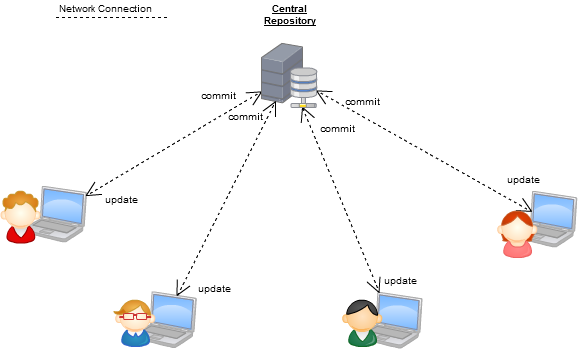
\includegraphics[width=\linewidth]{figs/centralized.png}
	\column{.50\linewidth}
	\centering Distributed (Git)\\\smallskip
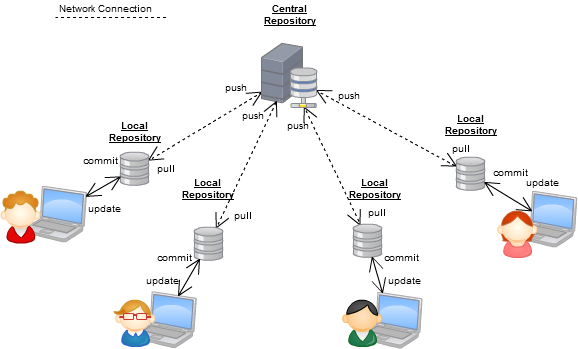
\includegraphics[width=\linewidth]{figs/distributed.png}
\end{columns}

\tiny \href{http://softwareengineering.stackexchange.com/questions/35074/im-a-subversion-geek-why-should-i-consider-or-not-consider-mercurial-or-git-or}{(Source)}
\end{center}
\end{frame}

%%%%%%%%%%%%%%%%%%%%%%%%%%%%%%%%%%%%%%%%%%%%%%%%%%%%%%%%%%%%%%%%%%%%%


\begin{frame}{Git}{Git vs. SVN (II)}
\begin{center}
\begin{columns}
	\column{.50\linewidth}
	\centering Fully distributed (Git)\\\smallskip
	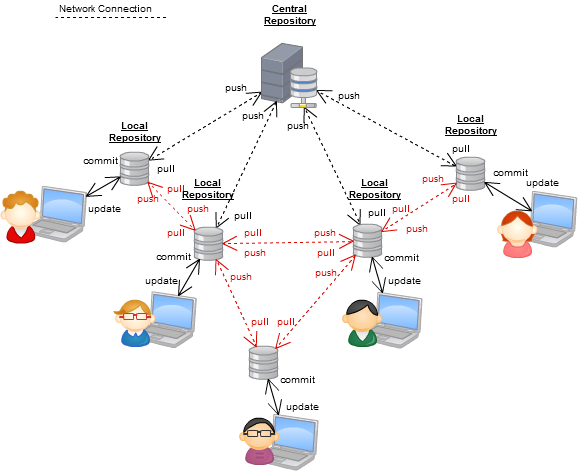
\includegraphics[width=\linewidth]{figs/fulldistributed.png}
	\tiny \href{http://softwareengineering.stackexchange.com/questions/35074/im-a-subversion-geek-why-should-i-consider-or-not-consider-mercurial-or-git-or}{(Source)}

	\column{.50\linewidth}
	\begin{block}{Git concepts to know}
	\begin{itemize}
	\item \texttt{commit}, \texttt{update}
	\item \texttt{push}, \texttt{pull}
	\item \texttt{origin}, \texttt{remote}
	\end{itemize}
	\end{block}
\end{columns}

\end{center}

\end{frame}


%%%%%%%%%%%%%%%%%%%%%%%%%%%%%%%%%%%%%%%%%%%%%%%%%%%%%%%%%%%%%%%%%%%%%%
\section{Using Git}

%%%%%%%%%%%%%%%%%%%%%%%%%%%%%%%%%%%%%%%%%%%%%%%%%%%%%%%%%%%%%%%%%%%%%%
\subsection{Repository initialization and clonning}

%%%%%%%%%%%%%%%%%%%%%%%%%%%%%%%%%%%%%%%%%%%%%%%%%%%%%%%%%%%%%%%%%%%%%%

\begin{frame}[fragile]{Using Git}{Basic commands: Repository initialization}

When using Git for the first time:

\begin{verbatim}
git config --global user.email user@uah.es 
git config --global user.name  "Jane Doe"
\end{verbatim}

Initialization:

\begin{verbatim}
mkdir /path/to/your/project
cd /path/to/your/project
git init
git remote add origin https://<where>/<path>/<project.git>
git push -u origin --all # pushes up the repo and its refs for the first time
\end{verbatim} 

\end{frame}

%%%%%%%%%%%%%%%%%%%%%%%%%%%%%%%%%%%%%%%%%%%%%%%%%%%%%%%%%%%%%%%%%%%%%%
\begin{frame}{Using Git}{Basic commands: Repository clonning}

To work with someone else’s repository, we first need to \emph{clone} it to get a
local copy.

\texttt{git clone <repo>}

E.g.:

\texttt{git clone https://github.com/danrodgar/gitSlides.git}

\begin{footnotesize}Note: once cloned, you can edit the repository as much as you want. No changes make their way back to the ‘central’ repository until you explicitly do so.
\end{footnotesize}
\end{frame}


%%%%%%%%%%%%%%%%%%%%%%%%%%%%%%%%%%%%%%%%%%%%%%%%%%%%%%%%%%%%%%%%%%%%%%
\subsection{Basic commands}


\begin{frame}[fragile]{Using Git}{Basic commands: tracking files}

Then, we can start tracking files. To do so, we need to \texttt{add}, \texttt{commit}, and \texttt{push} the file(s) that we want to track.


\begin{verbatim}
echo "A new file..." >> Readme.md
git add Readme.md
git commit -m 'Initial commit'
git push -u origin master
\end{verbatim}

\end{frame}


%%%%%%%%%%%%%%%%%%%%%%%%%%%%%%%%%%%%%%%%%%%%%%%%%%%%%%%%%%%%%%%%%%%%%%
\begin{frame}{Using Git}{Basic commands: Pulling}

% \begin{columns}
% 	\column{.50\linewidth}
% 	\centering Centralized (SVN)\\\smallskip
% 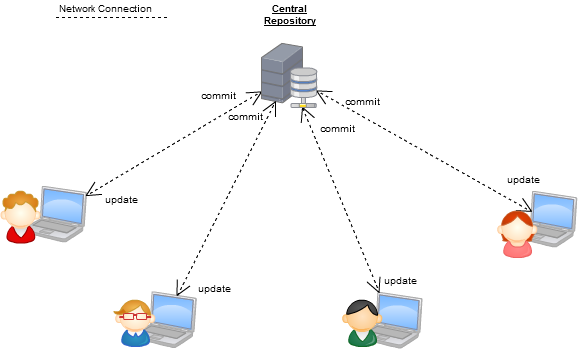
\includegraphics[width=\linewidth]{figs/centralized.png}
% 	\column{.50\linewidth}
% 	\centering Distributed (Git)\\\smallskip
% 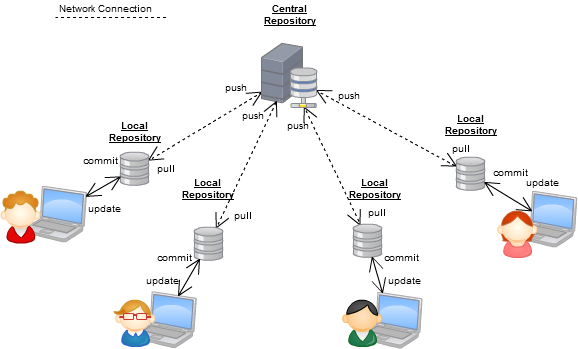
\includegraphics[width=\linewidth]{figs/distributed.png}
% \end{columns}
% To integrate all changes other people have made since you
% cloned/pulled: \texttt{git pull}

\begin{itemize}
 \item If you have made local changes you have to \\
 \texttt{git stash} \\
 before pulling, then \\
 \texttt{git stash pop} \\
 afterwards
 
 \item You can see which files you've modified with\\
  \texttt{git status}
 
 \item You can permanently remove your local changes by \\
 \texttt{git checkout <file>}
\end{itemize}

\end{frame}


%%%%%%%%%%%%%%%%%%%%%%%%%%%%%%%%%%%%%%%%%%%%%%%%%%%%%%%%%%%%%%%%%%%%%%
\begin{frame}{Using Git}{Basic commands: Pushing}

\texttt{git add <file>} makes git track the file <file> 

Or to record all changes into a commit (notice the ‘.’):

\texttt{git commit .} 

\texttt{git push origin master} This pushes all new commits to the repository.


\end{frame}


%%%%%%%%%%%%%%%%%%%%%%%%%%%%%%%%%%%%%%%%%%%%%%%%%%%%%%%%%%%%%%%%%%%%%%
\subsection{Merge and conflicts}
\begin{frame}{Using Git}{Merge and conflicts}

If two people both modify the same file, the first to push \emph{wins}.
The second person will have to pull and merge before pushing.

\begin{itemize}
 \item Changes in different parts of a file are automatically merged
 \item Changes in the same part of a file cause conflicts (between <<<
=== >>> ) and require the user to manually resolve them. Can
select either HEAD (your changes) or remote, or a mix of the two
\item Two merging cases: have / haven't committed
\end{itemize}

\end{frame}

%%%%%%%%%%%%%%%%%%%%%%%%%%%%%%%%%%%%%%%%%%%%%%%%%%%%%%%%%%%%%%%%%%%%%%
\begin{frame}{Using Git}{Merge and conflicts: \texttt{diff}}

\texttt{diff -u <old file> <new file>} 

This command shows what changes you would need to apply to old file to change it into
new file.

Lines beginning with:
\begin{itemize}
 \item \texttt{- - -} or \texttt{+++} tell you the old / new filenames
 \item \texttt{@@} points to where within the file you are looking \\
       (i.e. a space) are lines that are unchanged
 \item \texttt{-} is a deleted line
 \item \texttt{+} is a newly added line
\end{itemize}

\end{frame}



%%%%%%%%%%%%%%%%%%%%%%%%%%%%%%%%%%%%%%%%%%%%%%%%%%%%%%%%%%%%%%%%%%%%%%
\begin{frame}[fragile]{Using Git}{Merge and conflicts: \texttt{diff} example}

\begin{scriptsize}
\begin{columns}
	\column{.50\linewidth}
	  \begin{verbatim}
	  #include <stdio.h> 
	  int main() {
	    printf("Hello World\n");
	  }
	  \end{verbatim}
	\column{.50\linewidth}
	  \begin{verbatim}
	    #include <stdio.h>
	    int main(int argc, char *argv[]) {
	    printf("Hello World\n");
	    return 0;
	    }
	  \end{verbatim}
\end{columns}

Applying the \texttt{diff} command:
\begin{verbatim}
$ diff -u hello.c hello_new.c > hello.patch
\end{verbatim}

We get the following patch:
\begin{verbatim}
--- hello.c	2014-10-07 18:17:49.000000000 +0530
+++ hello_new.c	2014-10-07 18:17:54.000000000 +0530
@@ -1,5 +1,6 @@
 #include <stdio.h>
-int main() {
+int main(int argc, char *argv[]) {
 	printf("Hello World\n");
+	return 0;
 }
\end{verbatim}
\end{scriptsize}


\end{frame}

%%%%%%%%%%%%%%%%%%%%%%%%%%%%%%%%%%%%%%%%%%%%%%%%%%%%%%%%%%%%%%%%%%%%%%

\begin{frame}{Using Git}{Merge and conflicts: Applying \texttt{diff} changes (patch command)}

After the \texttt{patch.diff} is created as:

\texttt{diff -u <old file> <new file> > file.patch }

We can apply it with the \texttt{patch} command:

\texttt{patch < file.patch}

Note that the \texttt{file.patch} knows the name of the file to be patched.


\end{frame}

%%%%%%%%%%%%%%%%%%%%%%%%%%%%%%%%%%%%%%%%%%%%%%%%%%%%%%%%%%%%%%%%%%%%%%

\begin{frame}{Using Git}{Merge and conflicts: Original Patch!}

\centering
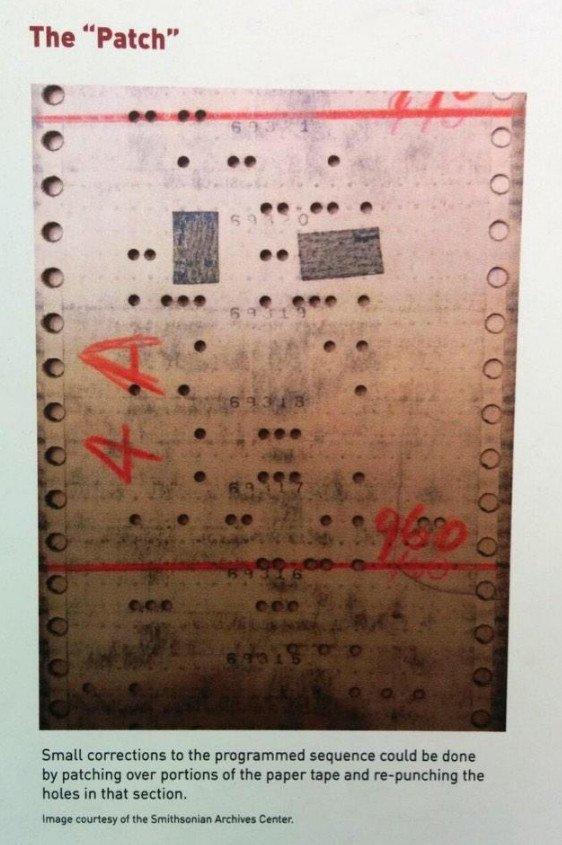
\includegraphics[width=.4\textwidth,height=\textheight,keepaspectratio]{figs/patch.png}

\end{frame}


%%%%%%%%%%%%%%%%%%%%%%%%%%%%%%%%%%%%%%%%%%%%%%%%%%%%%%%%%%%%%%%%%%%%%%
\begin{frame}{Using Git}{Commits}

\begin{itemize}
 \item Merge commits record where parallel development unified
 \item How does Git keep track of things when parallel development
happens?
\item Every commit has an ID (its hash), which is a 40 character SHA-1
hash based on the commit's content. Not guaranteed to be
unique; but it probably is
\end{itemize}

\end{frame}

%%%%%%%%%%%%%%%%%%%%%%%%%%%%%%%%%%%%%%%%%%%%%%%%%%%%%%%%%%%%%%%%%%%%%%
\subsection{Branches}
\begin{frame}{Using Git}{Branches}

Branches are used extensively (e.g. some like feature branches).

\begin{itemize}
 \item A repository (local and remote) can have explicit branches
 \item The default branch is called master
 \item \texttt{git branch <name>} creates branches
 \item \texttt{git checkout <branch name>} switch branches
 \item To merge branch X into Y, checkout Y and run git merge X
(i.e. you say “I want to merge another branch into me”)
\end{itemize}

\end{frame}

%%%%%%%%%%%%%%%%%%%%%%%%%%%%%%%%%%%%%%%%%%%%%%%%%%%%%%%%%%%%%%%%%%%%%%
% \subsection{Tags}
% \begin{frame}{Using Git}{Tags}
% 	TODO
% \end{frame}

%%%%%%%%%%%%%%%%%%%%%%%%%%%%%%%%%%%%%%%%%%%%%%%%%%%%%%%%%%%%%%%%%%%%%%
\subsection{Advanced Git}
\begin{frame}{Using Git}{Advanced Git: Getting an old commit}

Sometimes you need to get an old file or discard some changes. With 

\begin{itemize}
 \item \texttt{git log} 
 \item \texttt{git log -- oneline}
\end{itemize}

we can check previous commits and select one with \texttt{checkout}, e.g.:
\begin{itemize}
 \item \texttt{git checkout c71d008}
\end{itemize}

\end{frame}


%%%%%%%%%%%%%%%%%%%%%%%%%%%%%%%%%%%%%%%%%%%%%%%%%%%%%%%%%%%%%%%%%%%%%%
\begin{frame}{Using Git}{Advanced Git: Good practices}


Tipically changes are checked by someone other than their
author before being merged into master. This kind of \textbf{code review} is is naturally captured by pull requests in Git.

Learn on the job: the best way to learn it is by using it. However:
\begin{itemize}
  \item Best practice: regularly push and pull (at least daily, in general).
  \item Don't push half-baked changes or pull if you're in the middle of a task.
\end{itemize}

\end{frame}

%%%%%%%%%%%%%%%%%%%%%%%%%%%%%%%%%%%%%%%%%%%%%%%%%%%%%%%%%%%%%%%%%%%%%%

\section{GitHub}
\begin{frame}{GitHub}{GitHub}

\centering

\includegraphics[width=\textwidth,height=\textheight,keepaspectratio]{figs/github.png}


\end{frame}


% %%%%%%%%%%%%%%%%%%%%%%%%%%%%%%%%%%%%%%%%%%%%%%%%%%%%%%%%%%%%%%%%%%%%%%
% \begin{frame}{}
% 
% \end{frame}
% 


%%%%%%%%%%%%%%%%%%%%%%%%%%%%%%%%%%%%%%%%%%%%%%%%%%%%%%%%%%%%%%%%%%%%%%

\end{document}





